%%%%%%%%%%%%%%%%%%%%%%%%%%%%%%%%%%%%%%%%%
% Short Sectioned Assignment
% LaTeX Template
% Version 1.0 (5/5/12)
%
% This template has been downloaded from:
% http://www.LaTeXTemplates.com
%
% Original author:
% Frits Wenneker (http://www.howtotex.com)
%
% License:
% CC BY-NC-SA 3.0 (http://creativecommons.org/licenses/by-nc-sa/3.0/)
%
%%%%%%%%%%%%%%%%%%%%%%%%%%%%%%%%%%%%%%%%%

%----------------------------------------------------------------------------------------
%	PACKAGES AND OTHER DOCUMENT CONFIGURATIONS
%----------------------------------------------------------------------------------------

\documentclass[paper=a4, fontsize=11pt]{scrartcl} % A4 paper and 11pt font size
\usepackage{listings}
\usepackage[T1]{fontenc} % Use 8-bit encoding that has 256 glyphs
\usepackage{fourier} % Use the Adobe Utopia font for the document - comment this line to return to the LaTeX default
\usepackage[english]{babel} % English language/hyphenation
\usepackage{amsmath,amsfonts,amsthm} % Math packages
\usepackage{xeCJK}

\usepackage{lipsum} % Used for inserting dummy 'Lorem ipsum' text into the template

\usepackage{sectsty} % Allows customizing section commands
\allsectionsfont{\centering \normalfont\scshape} % Make all sections centered, the default font and small caps

\usepackage{fancyhdr} % Custom headers and footers
\pagestyle{fancyplain} % Makes all pages in the document conform to the custom headers and footers
\fancyhead{} % No page header - if you want one, create it in the same way as the footers below
\fancyfoot[L]{} % Empty left footer
\fancyfoot[C]{} % Empty center footer
\fancyfoot[R]{\thepage} % Page numbering for right footer
\renewcommand{\headrulewidth}{0pt} % Remove header underlines
\renewcommand{\footrulewidth}{0pt} % Remove footer underlines
\setlength{\headheight}{13.6pt} % Customize the height of the header

\numberwithin{equation}{section} % Number equations within sections (i.e. 1.1, 1.2, 2.1, 2.2 instead of 1, 2, 3, 4)
\numberwithin{figure}{section} % Number figures within sections (i.e. 1.1, 1.2, 2.1, 2.2 instead of 1, 2, 3, 4)
\numberwithin{table}{section} % Number tables within sections (i.e. 1.1, 1.2, 2.1, 2.2 instead of 1, 2, 3, 4)

\setlength\parindent{0pt} % Removes all indentation from paragraphs - comment this line for an assignment with lots of text

%----------------------------------------------------------------------------------------
%	TITLE SECTION
%----------------------------------------------------------------------------------------

\newcommand{\horrule}[1]{\rule{\linewidth}{#1}} % Create horizontal rule command with 1 argument of height

\title{	
\normalfont \normalsize 
\textsc{Fudan University} \\ [25pt] % Your university, school and/or department name(s)
\horrule{0.5pt} \\[0.4cm] % Thin top horizontal rule
\huge Computer Vision Report \\ % The assignment title
\horrule{2pt} \\[0.5cm] % Thick bottom horizontal rule
}

\author{杨越 13307130265} % Your name

\date{\normalsize\today} % Today's date or a custom date
\setlength{\parindent}{4em}
\setlength{\parskip}{1em}
\renewcommand{\baselinestretch}{2.0}

\begin{document}

\maketitle % Print the title

%----------------------------------------------------------------------------------------
%	PROBLEM 1
%----------------------------------------------------------------------------------------

\section{INTRODUCTION}

在计算机视觉领域,图像分割(Segmentation)指的是将数字图像细分为多个图像子区域(像素的集合)(也被称作超像素)的过程。

图像分割的目的是简化或改变图像的表示形式,使得图像更容易理解和分析。图像分割通常用于定位图像中的物体和边界(线,曲线等)。

更精确的,图像分割是对图像中的每个像素加标签的一个过程,这一过程使得具有相同标签的像素具有某种共同视觉特性。

图像分割的结果是图像上子区域的集合(这些子区域的全体覆盖了整个图像),或是从图像中提取的轮廓线的集合(例如边缘检测)。
一个子区域中的每个像素在某种特性的度量下或是由计算得出的特性都是相似的,例如颜色、亮度、纹理。邻接区域在某种特性的度量下有很大的不同。

\section{Mutiple Methods}

\begin{itemize}
\item Thresholding
\item Clustering methods
\item Compression-based methods
\item Histogram-based methods
\item Edge detection
\item Dual clustering method
\item Region-growing methods
\item Partial differential equation-based methods
\item Variational methods
\item Graph partitioning methods

\end{itemize}

\section{Efficient Graph-Based Image Segmentation}

\subsection{INTRODUCTION}

这是一篇经典的论文,能做出非常良好的分割效果。主要的思想是通过设定权值,将一个网格图分割成若干个联通块。

这个做法的效率也十分的可观。经测试180K的像素点只需要0.04s就可以分割出来.

\subsection{DEFINITION}


	\subsubsection{INternal difference}

	$$Int(C) = \max\limits_{e \in MST(C, E)} w(e)$$

	\subsubsection{Difference between two components}

	$$Dif(C_1, C_2) = \min\limits_{v_i \in C_1, v_j \in C_2, (v_i, v_j) \in E} w((v_i, v_j))$$

	如果没有边连接$(C_1, C_2)$, 则$Diff(C_1, C_2) = \infty$

	\subsection{Minimum internal difference}

	$$MInt(C_1, C_2) = min(Int(C_1) + \tau(C_1), Int(C_2) + \tau(C_2))$$

	$$\tau(C) = k / |C|$$

	\subsubsection{Predicate D}

	预测算子$D$, 用来决定是否两个联通块之间在一种分割中被分割开来。


	\begin{equation}
	D(C_1, C_2) = 
	\begin{cases}
	TRUE & \mbox{if $Diff(C_1, C_2) > MInt(C_1, C_2)$}\\
	FALSE & \mbox{otherwise}
	\end{cases}
	\end{equation}	

\subsection{Properties}
	
	因为存在我们的预测算子$D$, 如果$D$给出的结果是$FALSE$说明这个两个联通块不需要进行分割。\\
	由于$Dif(C_1, C_2)$和$MInt(C_1, C_2)$都是一个求最小值的过程, 因此, 如果确定了$(C_1, C_2)$处于一个联通块, $(C_2, C_3)$处于一个联通块, 那么$(C_1, C_3)$一定处于一个相同的联通块。

\subsection{ALGORITHM}

	\subsubsection{GAUSSIAN FILTER}
		对整个数字图像进行以输入的$\sigma$作为参数的Gaussian filter, 便于之后进行的处理。
	\subsubsection{Build Graph}
		将相邻的两个像素点, 以高斯模糊后的RGB值差的平方作为权值。建出一个网格图 $ G = (V, E) $
	\subsubsection{SEGMENTATION}
		\begin{enumerate}
			\item 对E的权值从小到大进行排序
			\item 从每个联通只包含本身的一个像素的点$S^0$开始.
			\item 对每条边按顺序执行下一步的算法.
			\item 由$S^{q-1}$构建下一步的$S^{q}$. 假设$V_i, V_j$是第$q$条边连接的两个点, $C_i^{q-1}$表示在$S^{q-1}$中$V_i$处于的联通块, $C_j^{q-1}$表示$S^{q-1}$中$V_j$处于的联通块.
				如果$C_i^{q-1} \neq C_j^{q-1}$, 并且$w(e_q) \leq MInt(C_i^{q-1}, C_j^{q-1})$, 那么合并$C_i^{q-1}$和$C_j^{q-1}$
			\item 最终的分割就是$S^q$
		\end{enumerate}

\subsection{RESULT AND EXPAMPLE}
\setlength{\parindent}{0em}
	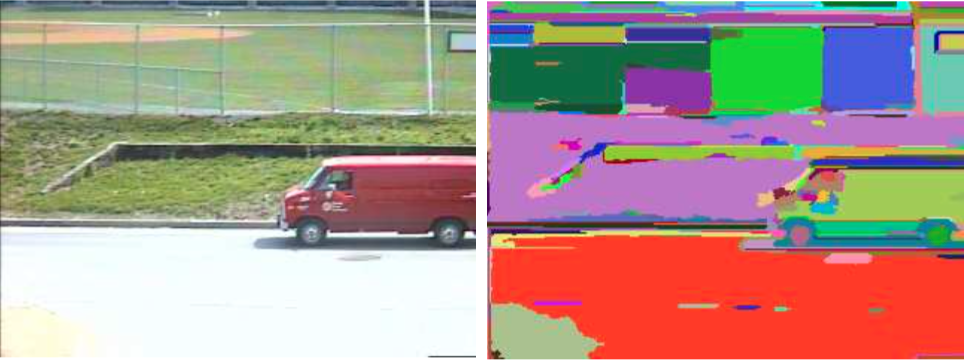
\includegraphics[scale=0.5]{pic1.png}

	Figure 1: $(320 \times 240)$ color image, with $(\sigma = 0.8, k = 300)$

	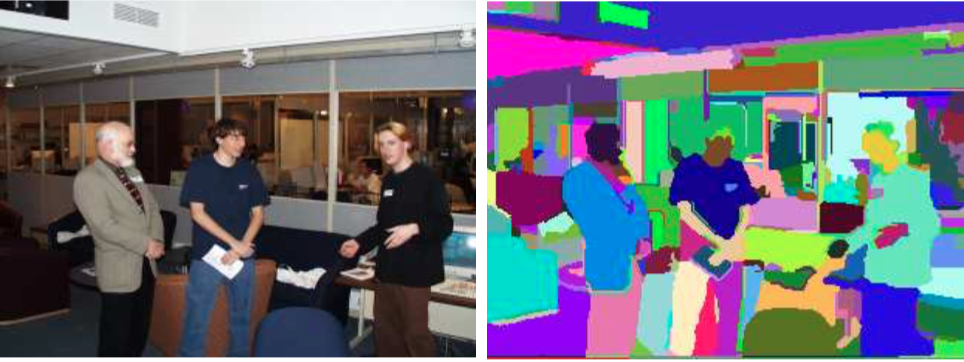
\includegraphics[scale=0.5]{pic2.png}

	Figure 2: $(320 \times 240)$ color image, with $(\sigma = 0.8, k = 300)$

	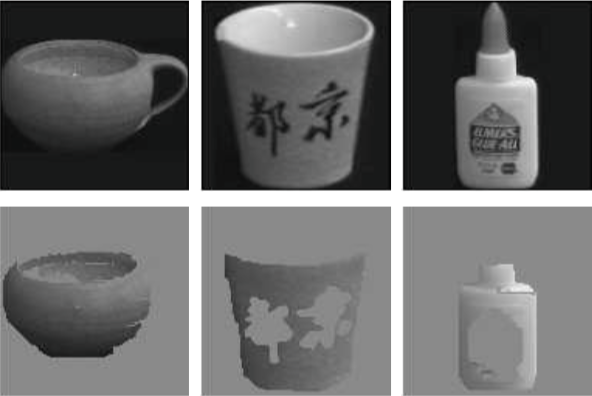
\includegraphics[scale=0.5]{pic3.png}

	Figure 3: $(128 \times 128)$ color image, with $(\sigma = 0.8, k = 150)$


\setlength{\parindent}{4em}

\section{Normalized Cuts and Image Segmentation}

\subsection{INTRODUCTION}
	这篇论文更偏于数学,虽然都是求解图分割问题,但通过完全不同的角度求解。
	将图分割的最优化问题,用代数的算术式子表示出来,接着通过线性代数进行求解。

\subsection{DEFINITION AND COMPUTING}
	图$ G = (V, E)$, 可以被分割进两个不相交集合,$A, B, A \cup B = V, A \cap B = \emptyset$。
	割集$$cut(A, B) = \sum\limits_{u \in A, v \in B} w(u, v)$$
	全局最小割算法是一个众所周知的算法。\\
	然而最小割可能出现如下情况。

	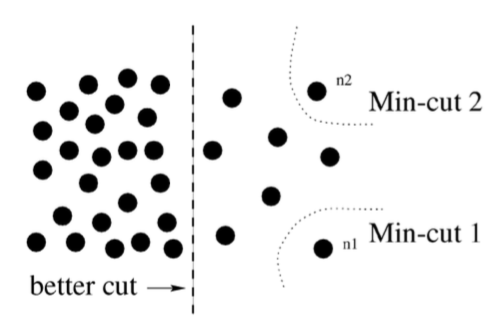
\includegraphics[scale=0.5]{pic4.png}

	Figure1, A case with minimum cut gives a bad partition.

	因此作者定义了新的估价函数 $Nomalized cut(Ncut)$
	$$Ncut(A, B) = \frac{cut(A, B)}{assoc(A, V)} + \frac{cut(A, B)}{assoc(B, V)}$$

	作者定义向量$\mathbf{x}, \mathbf{x}\in {-1, 1}^n$,$ -1$ 表示属于割集的$A$集合, $1$表示属于$B$集合. 

	令$$k = \frac{\sum_{xi>0} d_i}{\sum d_i}$$
	$$\mathbf{y = (1 + x) - b(1 - x)}$$

	\begin{align}
	\begin{split}
		Ncut(A, B) &= \frac{cut(A, B)}{assoc(A, V)} + \frac{cut(A, B)}{assoc(B, V)}	\\
			&= \frac{\sum_{x_i > 0, x_j < 0} w_{ij} x_i x_j}{\sum{x_i>0}d_i} + \frac{\sum_{x_i < 0, x_j > 0} -w_{ij} x_i x_j}{\sum_{x_i < 0} d_i}\\
			&= \frac{(1+\mathbf{x})^{T}(D-W)(1+\mathbf{x})}{k\mathbf{1}^{T}D\mathbf{1}} + \frac{(1-\mathbf{x})^{T}(D-W)(1-\mathbf{x})}{(1-k)\mathbf{1}^{T}D\mathbf{1}}
	\end{split}
	\end{align}

	因此 
	\begin{align}
	\begin{split}
		\min_{x}NCut(\mathbf{x}) &= \min_{y} \frac{\mathbf{y}^{T}(D-W)\mathbf{y}}{\mathbf{y}^{T}D\mathbf{y}}
	\end{split}
	\end{align}

	假设存在$\lambda$使得
	$$(D-W)\mathbf{y} = \lambda D\mathbf{y}$$

	那么带入式4.2, 
	$$\min_{x} NCut(x) = \lambda$$

	因此我们只需要求解特征值$\lambda$, 

	$$D^{-1/2}(D-W)D^{-1/2}z = \lambda z$$

	如此就将图分割最优化问题转换成为了求解矩阵特征值的问题。

\subsection{ALGORITHM}
	
	
	算出矩阵$D, W$。\\
	然后对于$D^{-1/2}(D-W)D^{-1/2}$求特征根. 这一部分利用牛顿迭代进行求解。\\
	找出最小的特征根, 根据特征根构造特征向量。\\
	根据特征向量确定每个像素点属于A集合还是B集合.\\
	递归的对两部分分割直到合适为止.

\subsection{RESULT AND EXAMPLE}
	
	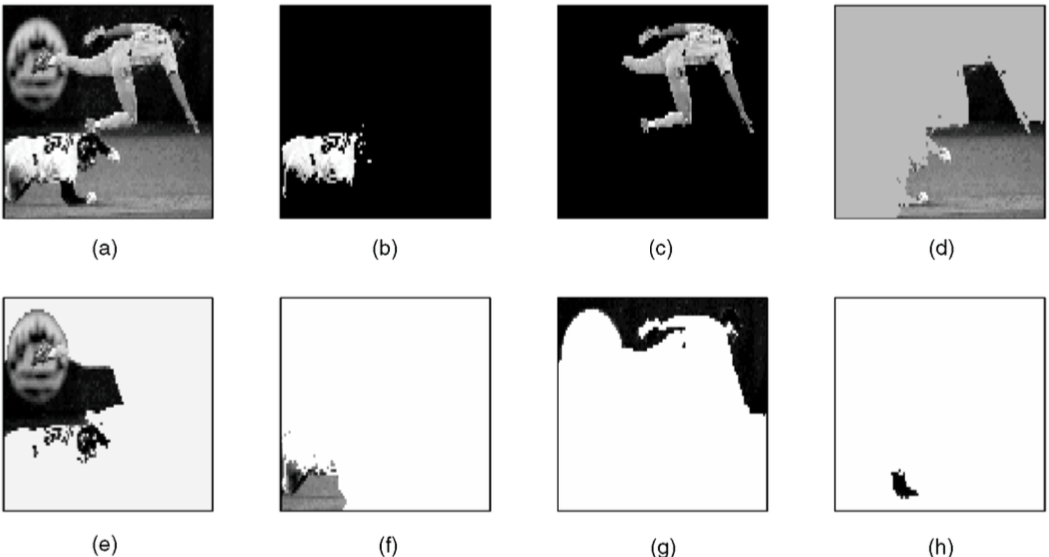
\includegraphics[scale=0.3]{pic5.png}

	Fig. 5. (a) shows the original image of size $80 \times  100$. Image intensity is normalized to lie within 0 and 1. Subplots (b)-(h) show the components of the partition with Ncut value less than 0.04.

	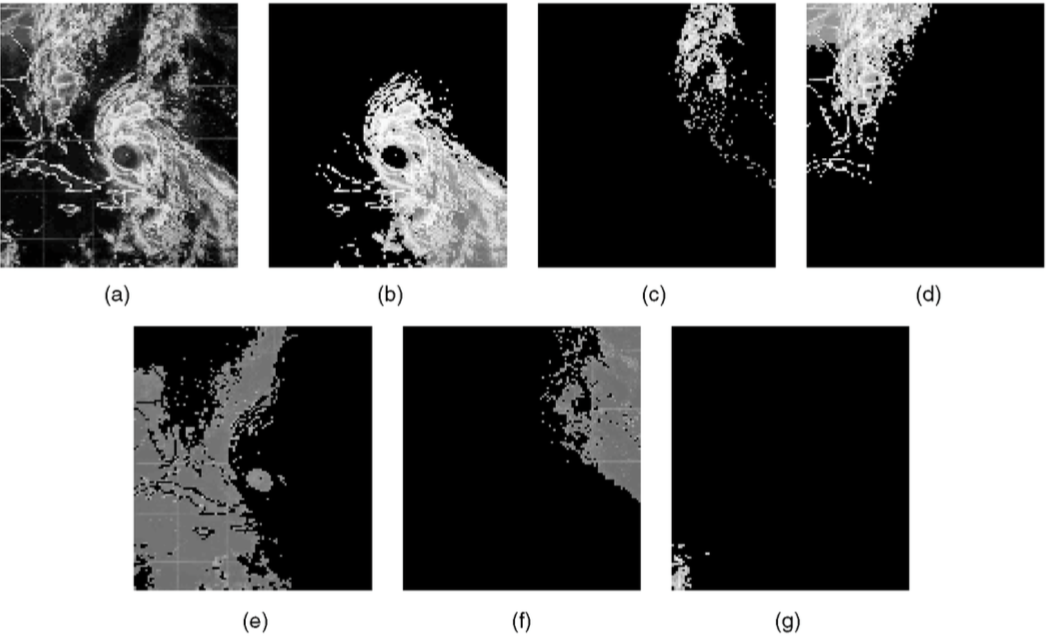
\includegraphics[scale=0.3]{pic6.png}

	Fig. 6. (a) shows a $126 \times  106 $ weather radar image. (b)-(g) show the components of the partition with Ncut value less than 0.08.

\section{Summary and conclustion}

可以看出两种算法的比较中, 第一种速度非常的快, 如果有$N$个像素点, 那么复杂的是$O(nlogn)$。而对于第二种则是$O(n^3)$. 然而第二种算法可以进行一部分比较粗糙的预处理, 先建立起某些联通块, 大大减小矩阵的大小.\\
因此最好的方法是两种方法结合, 先用第一种的方法算出一个比较粗略的segmentation, 利用求出的segmentation之后, 用第二种方法进行继续的求解. 达到一个更优解。

\end{document}